% Generated by code/variants/WritePaper.py from lazy-revision-interior-technical-v1.
\clearpage
\setcounter{figure}{0}
\renewcommand{\thefigure}{S\arabic{figure}}
\begin{center}
\begin{minipage}{\linewidth}
\captionsetup{type=figure,hypcap=false}
\centering
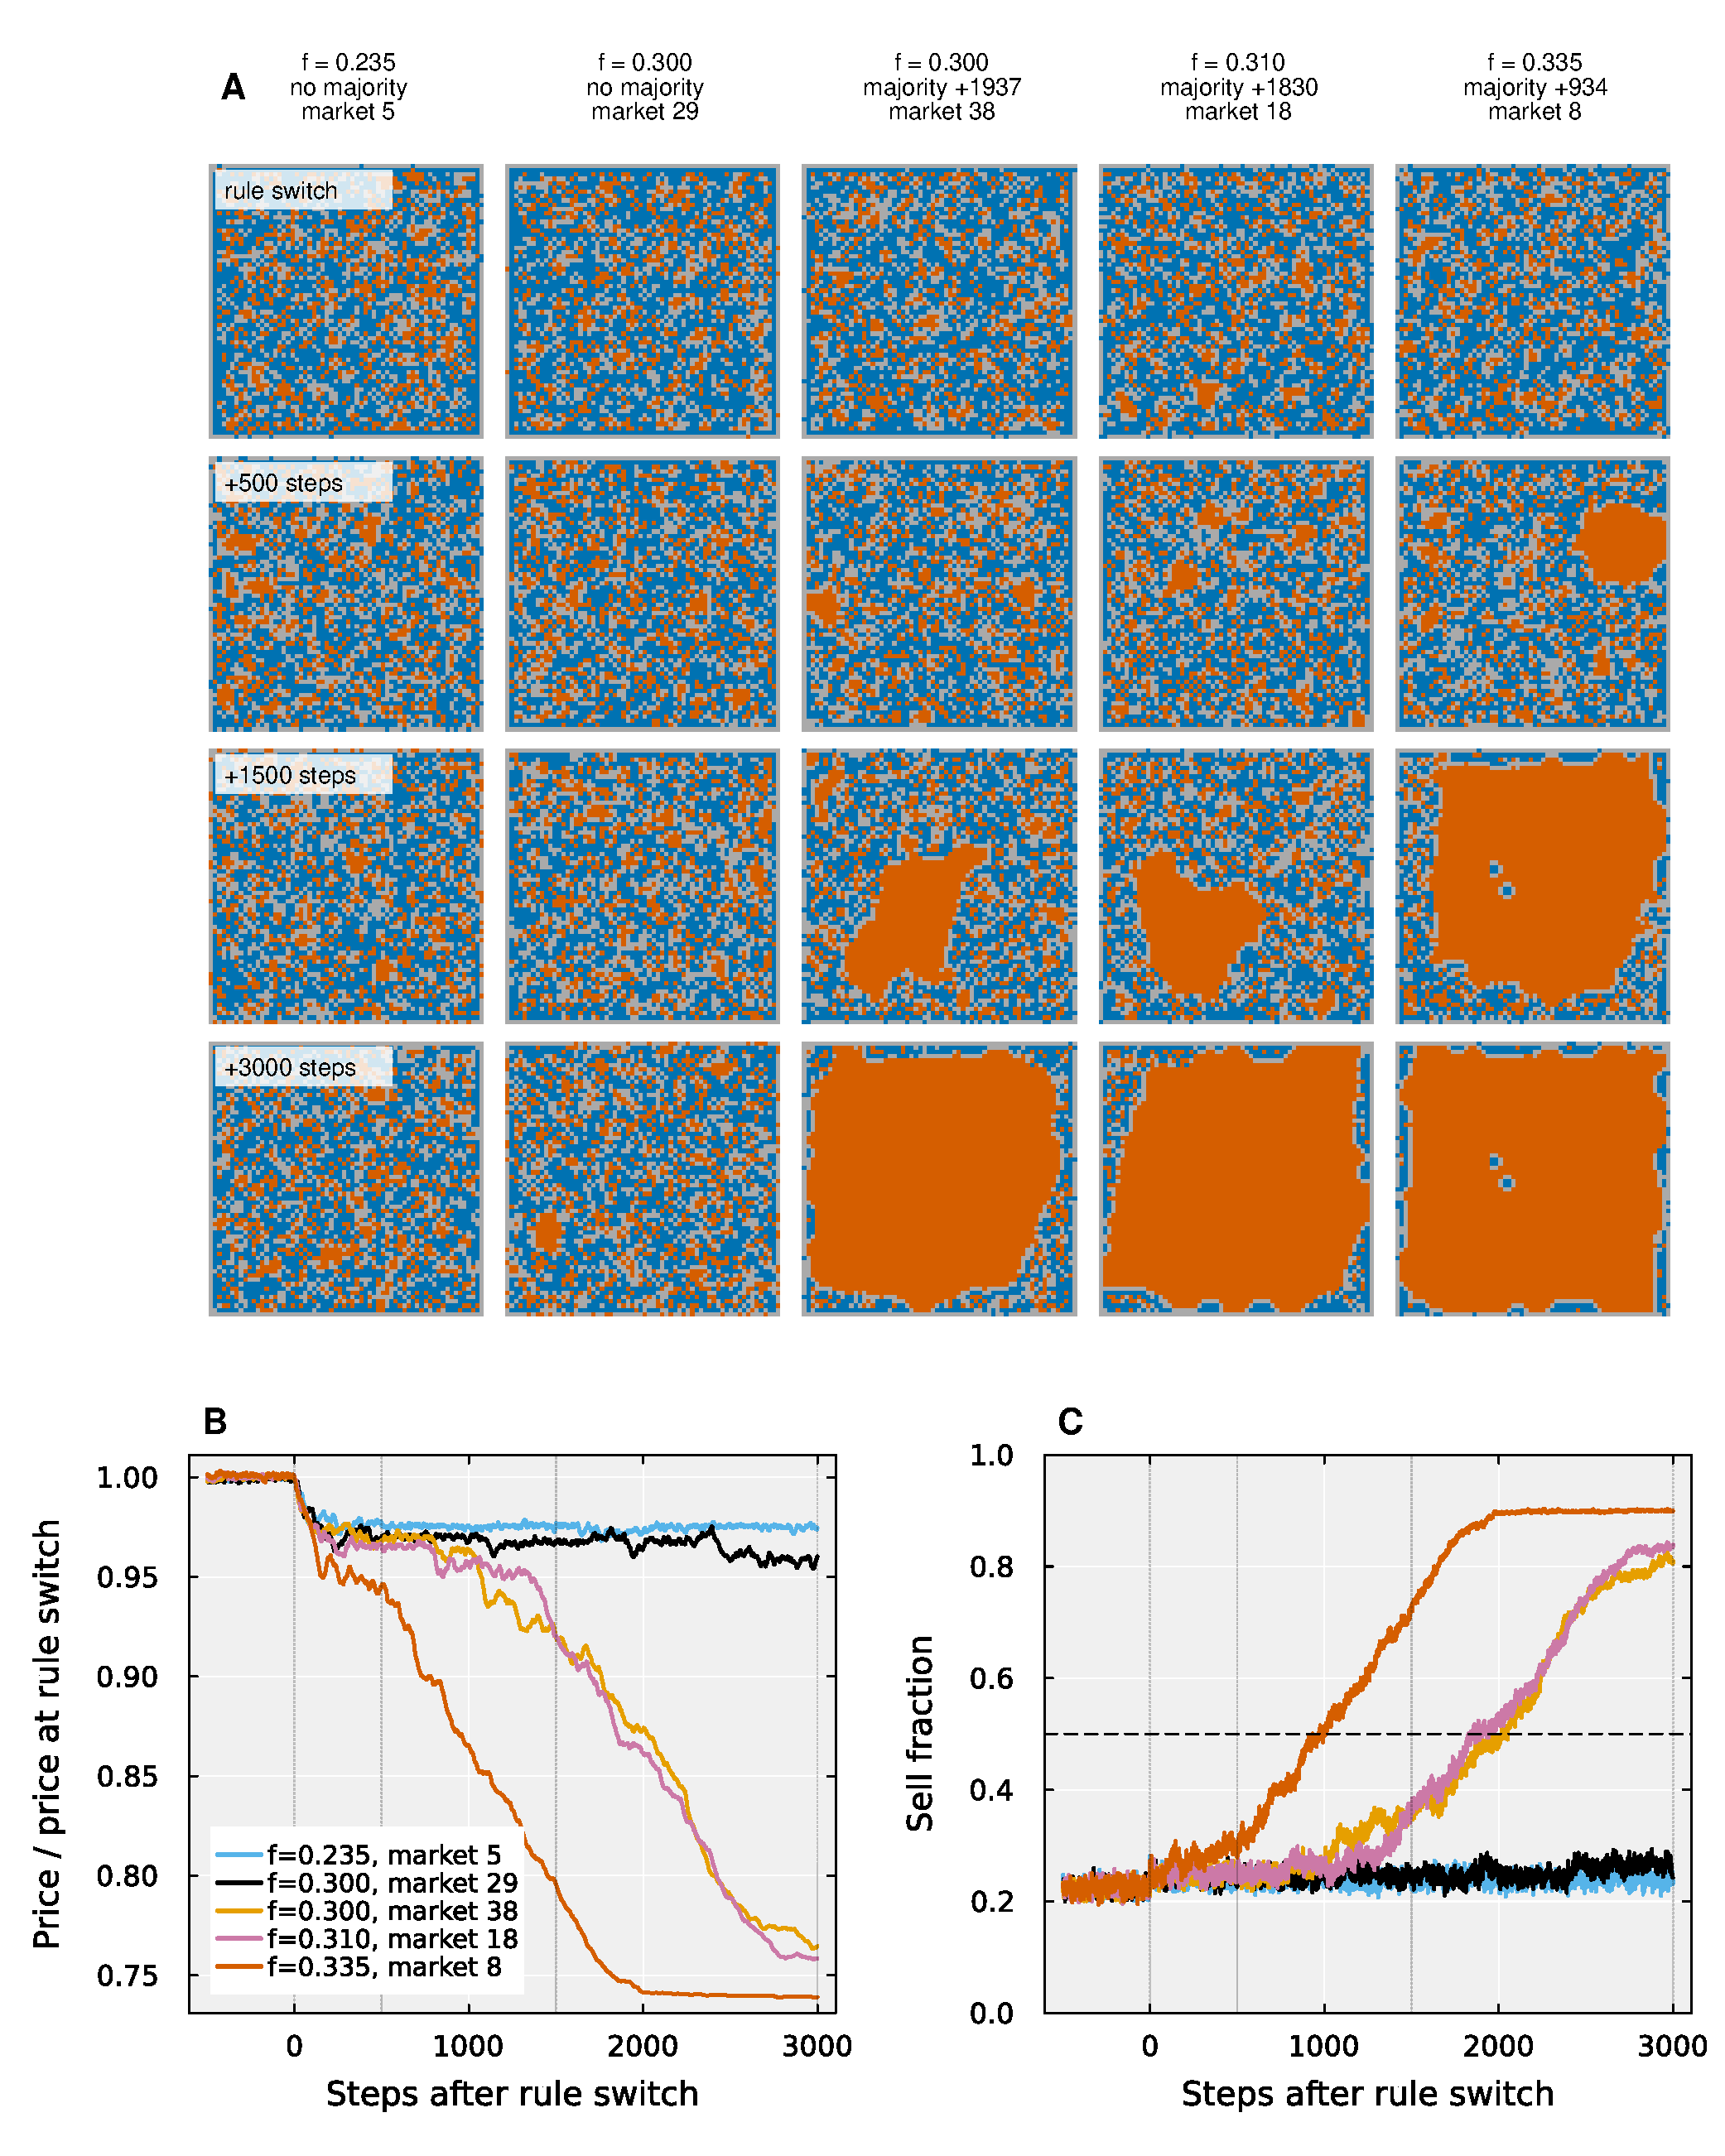
\includegraphics[width=0.87\linewidth]{figs/FigS1-RevisionMarketPanels.pdf}
\caption{Five example markets with revision probability $r=0.9$, active
technical traders, and dealer depth $h=100$ over 3,000 post-switch steps,
the counterpart of Fig.~\ref{fig:dose-panels} without the separate
checkerboard halves of the main model. Blue, gray, and orange denote Buy,
Hold, and Sell. The fractions $f=0.235$, 0.300, 0.310, and 0.335 were the tested
fractions whose majority probabilities at revision probability $r=0.9$ (0.00, 0.62, 0.84, and 1.00)
were nearest those of the fractions in Fig.~\ref{fig:dose-panels} at $r=1$
(0.00, 0.50, 0.84, and 1.00), with ties broken by proximity to the
$r=0.9$ midpoint. Within each fraction and outcome, the market nearest the
median onset, or the median final Sell fraction for markets without a
majority, was selected from the campaign summaries before any images were
inspected, with the starting-market number breaking ties.
\textbf{(A)}~Grid decisions at the rule switch and after 500, 1,500, and
3,000 steps. Starting markets were 5, 29, 38, 18, and 8, from left to right.
\textbf{(B)}~Quoted price divided by its value at the rule switch.
\textbf{(C)}~Interior Sell fraction, with one-half marked by a horizontal
line. Midpoints and widths appear in Supplementary
Table~\ref{tab:variants-timing}.}
\label{fig:variants-panels}
\end{minipage}
\end{center}
